\chapter{Design and Implementation}\label{chap:design}

The premise of this chapter is to describe the design, implementation and decisions taken during the development of the different programs that compose this project.

Section \ref{sec:general_program_design} describes the general design of the programs, and how they are divided. In \autoref{sec:sphere-object} and \autoref{sec:renderer}, we will see how the objects are designed and how the rendering is done, respectively. Then, \autoref{sec:output} describes how the output is generated and how it can be used to visualize the results of the ray-tracer and finally, the last section, \ref{sec:running_program}, describes how the program can be run and how to use the \texttt{Makefile} to run the program with different parameters.

\section{General Program Design}
\label{sec:general_program_design}
The "30,000 foot view" of the programs is a ray-tracer, that has multiple spheres, with different materials, indexes of refraction and sizes. Each of the pixels is calculated individually, and then, when all pixels have been processed, they are outputted to a \texttt{ppm} file.

As it can be inferred from the \autoref{fig:general_program_flow}, the program is divided into two main sections:
\begin{itemize}
    \item \textbf{Scene}: This section reads the input file and stores the spheres into their appropriate data-structures.
    \item \textbf{Renderer}: This section is the main loop of the program, processing each pixel and outputting the resulting image.
\end{itemize}

\begin{center}
\begin{figure}
  \begin{tikzpicture}[scale=0.7,transform shape,
                      >=Stealth, auto,
                      node distance=2cm]
    % Participants
    \node[draw,rectangle] (Main)         {Main};
    \node[draw,rectangle,right=of Main] (Camera)       {Camera};
    \node[draw,rectangle,right=of Camera] (HittableList) {HittableList};
    \node[draw,rectangle,right=of HittableList] (Sphere)       {Sphere};
    \node[draw,rectangle,right=of Sphere]     (Material)     {Material};

    % Lifelines
    \foreach \P in {Main,Camera,HittableList,Sphere,Material} {
      \draw[dotted] (\P.south) -- ++(0,-12cm);
    }

    % Messages
    \draw[->]
      ([yshift=-1cm] Main.south) --
      node[above]{Construct camera object}
      ([yshift=-1cm] Camera.south);

    \draw[->]
      ([yshift=-2cm] Main.south) --
      node[above]{Add Sphere(s)}
      ([yshift=-2cm] HittableList.south);

    \draw[->]
      ([yshift=-3cm] Main.south) --
      node[above]{Generate ray}
      ([yshift=-3cm] Camera.south);

    \draw[->]
      ([yshift=-4cm] Camera.south) --
      node[above]{Test ray intersection (hit)}
      ([yshift=-4cm] HittableList.south);

    \draw[->]
      ([yshift=-5cm] HittableList.south) --
      node[above]{Check for hit}
      ([yshift=-5cm] Sphere.south);

    \draw[dashed,->]
      ([yshift=-6cm] Sphere.south) --
      node[above]{Return hit result}
      ([yshift=-6cm] HittableList.south);

    \draw[dashed,->]
      ([yshift=-7cm] HittableList.south) --
      node[above]{Return closest hit}
      ([yshift=-7cm] Camera.south);

    \draw[dashed,->]
      ([yshift=-8cm] Camera.south) --
      node[above]{Return color}
      ([yshift=-8cm] Main.south);

    \draw[->]
      ([yshift=-9cm] Main.south) --
      node[above]{Compute scatter/reflection/refraction}
      ([yshift=-9cm] Material.south);

    \draw[dashed,->]
      ([yshift=-10cm] Material.south) --
      node[above]{Return scattered ray}
      ([yshift=-10cm] Main.south);

    % Self‐message loop
    \draw[->]
      ([yshift=-11cm] Main.south)
        .. controls +(.8,0) and +(.8,-1) ..
      node[right]{Output color}
      ([yshift=-12cm] Main.south);
  \end{tikzpicture}
\caption{General program data flow}
\label{fig:general_program_flow}
\end{figure}
\end{center}


\begin{figure}[]
    \centering
    \begin{multicols}{3}

        \textbf{C++ Implementation}
        \dirtree{%
        .1 ..
        .2 .clang-format.
        .2 .clang-tidy.
        .2 CMakeLists.txt.
        .2 src/.
        .3 camera.hpp.
        .3 color.hpp.
        .3 hittable\_list.hpp.
        .3 hittable.hpp.
        .3 image.hpp.
        .3 interval.hpp.
        .3 main.cpp.
        .3 material.hpp.
        .3 ray.hpp.
        .3 rtweekend.hpp.
        .3 sphere.hpp.
        .3 vec3.hpp.
        }
        
        \columnbreak
        
        \textbf{Go Implementation}
        \dirtree{%
        .1 ..
        .2 camera.go.
        .2 color.go.
        .2 go.mod.
        .2 hittable\_list.go.
        .2 hittable.go.
        .2 image.go.
        .2 interval.go.
        .2 main.go.
        .2 material.go.
        .2 ray-tracer.
        .2 ray.go.
        .2 rtweekend.go.
        .2 sphere.go.
        .2 vec3.go.
        }
        
        \columnbreak
        
        \textbf{Python Implementation}
        \dirtree{%
        .1 ..
        .2 camera.py.
        .2 color.py.
        .2 hittable.py.
        .2 image.py.
        .2 main.py.
        .2 material.py.
        .2 ray.py.
        .2 tree-py.txt.
        .2 utils.py.
        .2 vec3.py.
        }
        
    \end{multicols}
    \caption{File structures for Ray-Tracer implementations in different languages}
    \label{fig:raytracer-structures}
\end{figure}

We can observe in \autoref{fig:raytracer-structures}, there are the different files that compose each of the implementations of the ray-tracer, in C++, Go and Python. The file structure is similar in all three languages, as they must have an almost identical implementation.


\section{Scene}
\label{sec:scene}
This first section of the program reads the input file and stores the spheres into their appropriate data-structures, as we will see in \autoref{sec:sphere-object}. 

\subsection{Sphere\_data design}

To ensure the consistency between programs and runs, I decided to create a file that would specify the layout of all spheres, and include the parameters for the camera setting, position and render settings:
\begin{itemize}
    \item \textbf{ratio <width: double> <height: double>} $\Rightarrow{}$ Aspect ratio of the output image (width / height).
    \item \textbf{width <int>} $\Rightarrow{}$ The number of pixels for the width in the output image.
    \item \textbf{samplesPerPixel <int>} $\Rightarrow{}$ How many times each of the pixels is processed. The higher this number is, the slower the render, but the less noise that the output image has. See \autoref{fig:ray_traced_average} and \autoref{fig:ray_traced_max} for examples of the same image with different \texttt{samplesPerPixel} values.
    \item \textbf{maxDepth <int>} $\Rightarrow{}$ Specifies how many bounces a ray has to perform before getting the resulting color.
    \item \textbf{vfov <int>} $\Rightarrow{}$ State the \gls{fov} of the camera.
    \item \textbf{lookFrom <x: double> <y: double> <z: double>} $\Rightarrow{}$ Position of the camera in 3D space, where x is width, y is the height and z is the depth.
    \item \textbf{lookAt <x: double> <y: double> <z: double>} $\Rightarrow{}$ States the relative "up" orientation of the camera.
    \item \textbf{vup <x: double> <y: double> <z: double>} $\Rightarrow{}$ Vector that describes what is "up" in the scene
    \item \textbf{defocusAngle <double>} $\Rightarrow{}$ This parameter represents the "aperture". A higher number will mean more objects will be in focus, and a smaller number results in a shallower dept of field.
    \item \textbf{focusDist <double>} $\Rightarrow{}$ Specified the distance from camera look from point to a plane where the elements are in perfect focus
\end{itemize}

\subsection{Language Specific}
To try eliminating any possible influence of libraries created in other programming languages, all programs have been created only using their own standard library.

\subsubsection{C++}
When using C++, the intent was to use some of C++ modern features that would make development easier and adapted to new standards such as the use of smart pointers, \texttt{constexpr} and range-based loops. It was designed as an object-oriented program, with polymorphism though virtual functions (inside \texttt{material}, \texttt{hittable}).

The idea of making it header only was the benefits of inlining, easy to distribute and easily separable concepts and, as the compilation time is not crucial, the re-compilation of the headers every time there is a modification is not a drawback.

For multithreaded operations, I selected the \gls{openMP} library due to its ease of use and excellent performance. \gls{openMP} has been a widely adopted standard for decades, supported by most compilers, and originally emerged from the Fortran ecosystem in the 1960s.

\subsubsection{Go}
When choosing Go as to build the ray-tracer, as Go does not support inheritance like other \gls{oop} languages, I had to use \texttt{interfaces}, which are the tools Go provide for polymorphism. Interfaces are a type that defines a set of method signatures. Thus, for any struct that has the signature methods described in an interface, it can be called as an object from that type.

% --- GO CODE Interfaces ---
\begin{lstlisting}[language=Go, caption={Go interface example.}, label={lst:go_interface_example}
]
type Material interface {
	Scatter(rIn Ray, rec HitRecord) (bool, Color, Ray)
}

type Hittable interface {
	Hit(r Ray, rayT Interval, rec *HitRecord) bool
}
\end{lstlisting}

In my specific implementation, two instances of these keywords were used to denote all types of materials and all Hittable objects, that have to implement a scatter function and a hit function as described in \autoref{lst:go_interface_example}.

\subsubsection{Python}
Python is one of the most open languages, where there are many ways of developing the same program. There have been some problems with python's parameters in functions, whether they are passed as parameters or as references. Unlike in C++ where you can add \texttt{\&} to symbolize the passing the parameter by reference in the function signature, or using the \texttt{*} in Go, in Python, at first, it seems you can not specify this behavior. But if you research into the inner-workings of python functions and how they work, it seems that "Python passes function arguments by assigning to them" as \cite{python-names-pycon15} states at PyCon 2015:

\begin{lstlisting}[language=Python]
def augment_twice_bad(a_list, val):
    """Put val on the end of 'a_list' twice."""
    a_list = a_list + [val, val]

nums = [1, 2, 3]
augment_twice_bad(nums, 4)
print(nums)             # [1, 2, 3]
\end{lstlisting}

When calling the function \texttt{augment\_twice\_bad}, the parameters are assigned the values \texttt{nums} and \texttt{4} respectively. 

\begin{center}
\texttt{augment\_twice\_bad(nums, 4)}
\end{center}

\begin{center}
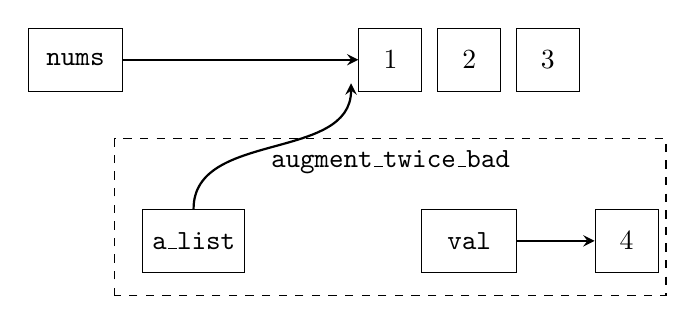
\begin{tikzpicture}[
    box/.style={rectangle, draw, minimum width=0.8cm, minimum height=0.8cm},
    varbox/.style={rectangle, draw, minimum width=1.2cm, minimum height=0.8cm},
    arrow/.style={->, >=stealth, thick}
]

% nums variable and list (outside function)
\node[varbox] (nums) at (-4, 1.5) {\texttt{nums}};
\node[box] (list1) at (0, 1.5) {1};
\node[box] (list2) at (1, 1.5) {2};
\node[box] (list3) at (2, 1.5) {3};

% Function frame (dashed rectangle)
\draw[dashed] (-3.5, -1.5) rectangle (3.5, 0.5);
\node at (0, 0.2) {\texttt{augment\_twice\_bad}};

% Function parameters
\node[varbox] (a_list) at (-2.5, -0.8) {\texttt{a\_list}};
\node[varbox] (val) at (1, -0.8) {\texttt{val}};
\node[box] (val_content) at (3, -0.8) {4};

% Arrows
\draw[arrow] (nums) -- (list1);
\draw[arrow] (a_list) to[out=90, in=270] (-0.5, 1.2);
\draw[arrow] (val) -- (val_content);

\end{tikzpicture}
\end{center}


The next statement is an assignment. The expression on the right-hand side makes a new list, which is then assigned to \texttt{a\_list} thus any further modification is made to the local variable only:

\begin{center}
\texttt{a\_list = a\_list + [val, val]}
\end{center}

\begin{center}
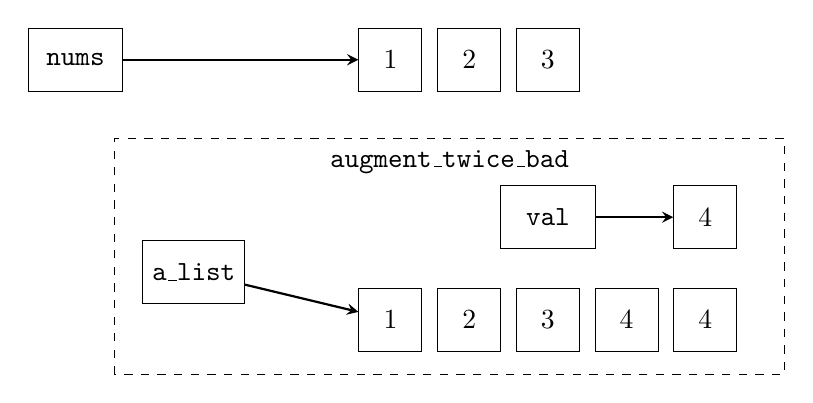
\begin{tikzpicture}[
    box/.style={rectangle, draw, minimum width=0.8cm, minimum height=0.8cm},
    varbox/.style={rectangle, draw, minimum width=1.2cm, minimum height=0.8cm},
    arrow/.style={->, >=stealth, thick}
]

% nums variable and original list (outside function)
\node[varbox] (nums) at (-4, 2.5) {\texttt{nums}};
\node[box] (orig1) at (0, 2.5) {1};
\node[box] (orig2) at (1, 2.5) {2};
\node[box] (orig3) at (2, 2.5) {3};

% Function frame (dashed rectangle)
\draw[dashed] (-3.5, -1.5) rectangle (5, 1.5);
\node at (0.75, 1.2) {\texttt{augment\_twice\_bad}};

% Function parameters
\node[varbox] (val) at (2, 0.5) {\texttt{val}};
\node[box] (val_content) at (4, 0.5) {4};

\node[varbox] (a_list) at (-2.5, -0.2) {\texttt{a\_list}};

% New list that a_list now points to
\node[box] (new1) at (0, -0.8) {1};
\node[box] (new2) at (1, -0.8) {2};
\node[box] (new3) at (2, -0.8) {3};
\node[box] (new4) at (3, -0.8) {4};
\node[box] (new5) at (4, -0.8) {4};

% Arrows
\draw[arrow] (nums) -- (orig1);
\draw[arrow] (a_list) -- (new1);
\draw[arrow] (val) -- (val_content);

\end{tikzpicture}
\end{center}

When the function ends, its local names are destroyed, and any values no longer referenced are reclaimed, leaving us just where we started:

\begin{center}
\texttt{print(nums)}
\end{center}

\begin{center}
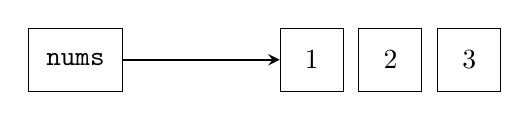
\begin{tikzpicture}[
    box/.style={rectangle, draw, minimum width=0.8cm, minimum height=0.8cm},
    varbox/.style={rectangle, draw, minimum width=1.2cm, minimum height=0.8cm},
    arrow/.style={->, >=stealth, thick}
]

% nums variable and list (back to original state)
\node[varbox] (nums) at (-2, 0) {\texttt{nums}};
\node[box] (list1) at (1, 0) {1};
\node[box] (list2) at (2, 0) {2};
\node[box] (list3) at (3, 0) {3};

% Arrow
\draw[arrow] (nums) -- (list1);

\end{tikzpicture}
\end{center}

\section{Object}
\label{sec:sphere-object}
All objects in this program are spheres, even the "ground" is a sphere with a big enough radius that it seems a plane.

\subsubsection{C++}
Each of the spheres in C++ is a class called \texttt{sphere}, as all objects in this scene are spheres. \texttt{sphere} is a derived class from \texttt{hittable}, an abstract class, such that in the case that, in the future the program is modified to have more objects, it is easily implemented. 

\begin{lstlisting}[language=C++, caption={Sphere Class for C++}, label={lst:sphere_cpp}]
class sphere : public hittable {
  public:
    sphere(point3 const & center, double radius,
           shared_ptr<material> mat)
      : center(center), radius(std::fmax(0, radius)), mat(mat) { }

    bool hit(ray const & r, interval ray_t,
             hit_record & rec) const override { ... }

  private:
    point3 center;
    double radius;
    shared_ptr<material> mat;
};
\end{lstlisting}



\subsubsection{Go}
Each of the spheres in Go is a struct, one for each of the materials implemented (Lambertian, Metal, Dielectric). Each of these types of materials implement the \texttt{Scatter} method, described in \autoref{lst:go_interface_example}.

\begin{lstlisting}[language=Go, caption={Go materials structs.}, label={lst:go_materials_structs}]
// Solid color
type Lambertian struct {
	Albedo Color
}

// Fuzz: 0 for perfect mirror, higher for fuzzier reflection
type Metal struct {
	Albedo Color
	Fuzz   float64 
}

// Transparent material such as water or ice
type Dielectric struct {
	RefractionIndex float64
}
\end{lstlisting}



\subsubsection{Python}
All spheres in Python are different classes that inherit from the same Material class:
\begin{lstlisting}[language=Python, caption={Python abscract class.}, label={lst:python_material_abstract}]
class Material(ABC):
    \@abstractmethod
    def scatter(self, r_in: Ray, rec: 'HitRecord') -> tuple[bool, Color, Ray]:
        """Returns (scatter_happened, attenuation, scattered_ray)"""
        
\end{lstlisting}
    


\section{Renderer}
\label{sec:renderer}
The main loop of the program is processing the object read from the file, added to the scene. 
This loop has two version in each of the programs designed:
\begin{itemize}
    \item \textbf{Single-threaded loop}: The program only runs using one core. It has a double loop where it processes all the pixels in the image, one by one. This is an extremely \gls{cpu} intensive process, as there are many pixels and iterations to go though each of those pixels. After all pixels are processed, they are outputted into the \texttt{output\_file}
    
    \item \textbf{multithreaded loop}: There are many ways a multithreaded renderer can work, even on different programming languages, different implementations have been chosen for specific reasons regarding their parallelization implementations. But in general, each of the pixels is processed, and then they are all joined into an array / list that is outputted to a file.
\end{itemize}


\subsection{Multiprocessing}
As previously stated, each of the programming languages, not only uses a different approach into how they have been parallelized, but even the algorithm had to be changed, as the implementation of python's interpreters makes the obvious parallelization perform surprisingly bad (this will be discussed in its section)

\subsubsection{C++}
To implement multiprocessing in C++, the \gls{openMP} library has been used, as it allows implementing parallelism with a low-effort compared to the great results it provides. 

\begin{lstlisting}[language=C++, caption={OpenMP Pragma instruction.}, label={lst:openmp_pragma}]
#pragma omp parallel for schedule(dynamic, 1) default(none)      \
    shared(image, world, lines_remaining, cout_mutex, std::cout) \
    firstprivate(samples_per_pixel, max_depth, image_width, image_height)
      for (int pixel = 0;
           pixel < image_width * image_height;
           pixel++) {
      ...
      }    
\end{lstlisting}

Dividing this \texttt{\#pragma} directive into its components to better understand why each of the sections exist and its effects on parallelizing:
\begin{itemize}
    \item \textbf{\#pragma omp parallel for}: This construct merges a parallel region with a for-loop, enabling work-sharing. Specifically, a group of threads is created, and all the iterations of the for-loop  are distributed among these threads.
    
    \item \textbf{schedule(dynamic, 1)}: Uses dynamic scheduling, meaning each thread grabs one job at a time. Using 1 creates some more scheduling overhead, but it ensures fine-grained balancing.
    
    \item \textbf{default(none)}: Disables all implicit data-sharing forcing the programmer to scope each variable used inside the parallel region. This helps at checking race conditions at compile time.
    
    \item \textbf{shared(image, world, lines\_remaining, cout\_mutex, std::cout)}: The named variables refer to a single instance in shared memory, visible to all threads:
    \begin{itemize}
        \item image: the pixel buffer, where all threads dump the processed pixel.
        \item World: the scene description, with all the spheres.
        \item Lines remaining: and atomic counter for progress reporting
        \item cout\_mutex + std::cout: Locking the cout\_mutex before writing to std::cout to serialize console output.
    \end{itemize}
    
    \item \textbf{firstprivate$(
    samples\_ per_pixel,
    max\_ depth,
    image\_ width,
    image\_ height)$}:
    Each thread has its own copy of these variables, with the values copied form the master thread, they are constants, read-only, although you can modify them locally, but they do not copy to other threads.
\end{itemize}

\subsubsection{Go}
To parallelize in go, its standard library provides a system called \glspl{goroutine}. These are "\glspl{green-thread}" that are created by Go's runtime every time the keyword \texttt{go} comes before a function.

\begin{lstlisting}[language=Go, caption={Goroutines.}, label={lst:go_goroutines_example}]
var wg sync.WaitGroup
waitChan := make(chan struct{}, numThreads)
lines_remaining := c.imageHeight

for pixel_idx := range c.imageHeight * c.ImageWidth {
    waitChan <- struct{}{}
    wg.Add(1)
    go func(pixel_idx int) { 
        defer wg.Done()
        ... 
        <-waitChan 
    }(pixel_idx)
}
wg.Wait()
    
\end{lstlisting}

To be able to limit the number of threads that can be created, a channel with a size of \texttt{numThreads} is created and each time a new \gls{goroutine} is going to be created, it tries to add a struct to the channel which, if there is an empty place, it adds the struct and allows the program to continue. But, if the channel is full, the program stops and does not allow any continuation of the program until the channel has a free spot, which is generated after the pixel is added to the resulting image.

To prevent the program from continue running before all the \glspl{goroutine} are finished, a \gls{wg} is used to prevent the main thread from continuing the main execution until all threads have finished (which is the same as the \gls{wg} being empty).

\subsubsection{Python}

To parallelize in python, I had to use the \texttt{concurrent.futures} library to properly parallelize the python execution.

This library can create two types of "executors" which are:
\begin{itemize}
    \item \textbf{ThreadPoolExecutor}: for \gls{i-o}-bound tasks (uses threads)
    \item \textbf{ProcessPoolExecutor}: for \gls{cpu}-bound tasks (uses processes)
\end{itemize}
To submit a task, you can use the following semantics, using python's list comprehension to create all the jobs:
\begin{lstlisting}[language=Python, caption={Python submiting jobs ProcessPoolExecutor.}, label={lst:python_executor_sumbit}]
futures = [
    executor.submit(self.process_row, j, world)
    for j in range(self.image_height)
]
\end{lstlisting}

This creates a job for every pixel, running the function \texttt{self.process\_row} inside the camera object, with parameters \texttt{j} and \texttt{world}.

To retrieve the results, you can simply iterate the futures object, as if it was a list of objects:
\begin{lstlisting}[language=Python, caption={Python retieving data from Process execution pool.}, label={lst:python_executor_retrieve}]
for future in futures:
    j, row_pixels = future.result()
    processed_rows += 1
    ...
    for i in range(self.image_width):
        img.set_pixel(i, j, row_pixels[i])
\end{lstlisting}


There is an interesting aspect on why the difference between the loops in Python and the rest of the programming languages: Compiled languages iterate over every pixel, while python iterates over every line, why is this? Because a copy of the entire python environment has to be created and the overhead of copying so much information slows down the program extremely. We will see the impact of these change in the evaluation section of the report.

\section{Output}
\label{sec:output}
The output of the program was initially thought to be though the standard output of the terminal, and redirecting the output to a \texttt{\gls{ppm}} file, but for measuring performance concerns and stability between different programs and their implementation of interacting with the operating system, it was decided that the program would create a file and output all the data into that file.

The design of the output is a \gls{ppm} file, in which the first three lines define the content, aspect and maximum values of a file. 
\begin{table}[H]
  \begin{tabular}{@{}ll@{}}
    \toprule
    Field        & Description                                 \\
    \midrule
    P3           & Magic number (P3 = ASCII, P6 = binary)      \\
    400 225      & Width and height (in pixels)                \\
    255          & Maximum color value                         \\
    \bottomrule
  \end{tabular}
  \caption{PPM file header fields}
  \label{tab:ppm-header}
\end{table}

In my specific case, I used P3, as I am outputting the \gls{rgb} values individually and a 255 maximum color value, to simplify the outputting of the resulting image.

This is an example image, of an image that this program would generate at maximum reasonable quality settings, 1920 width, 300 samples per pixel and 200 max depth.

\begin{figure}[h]
    \centering
    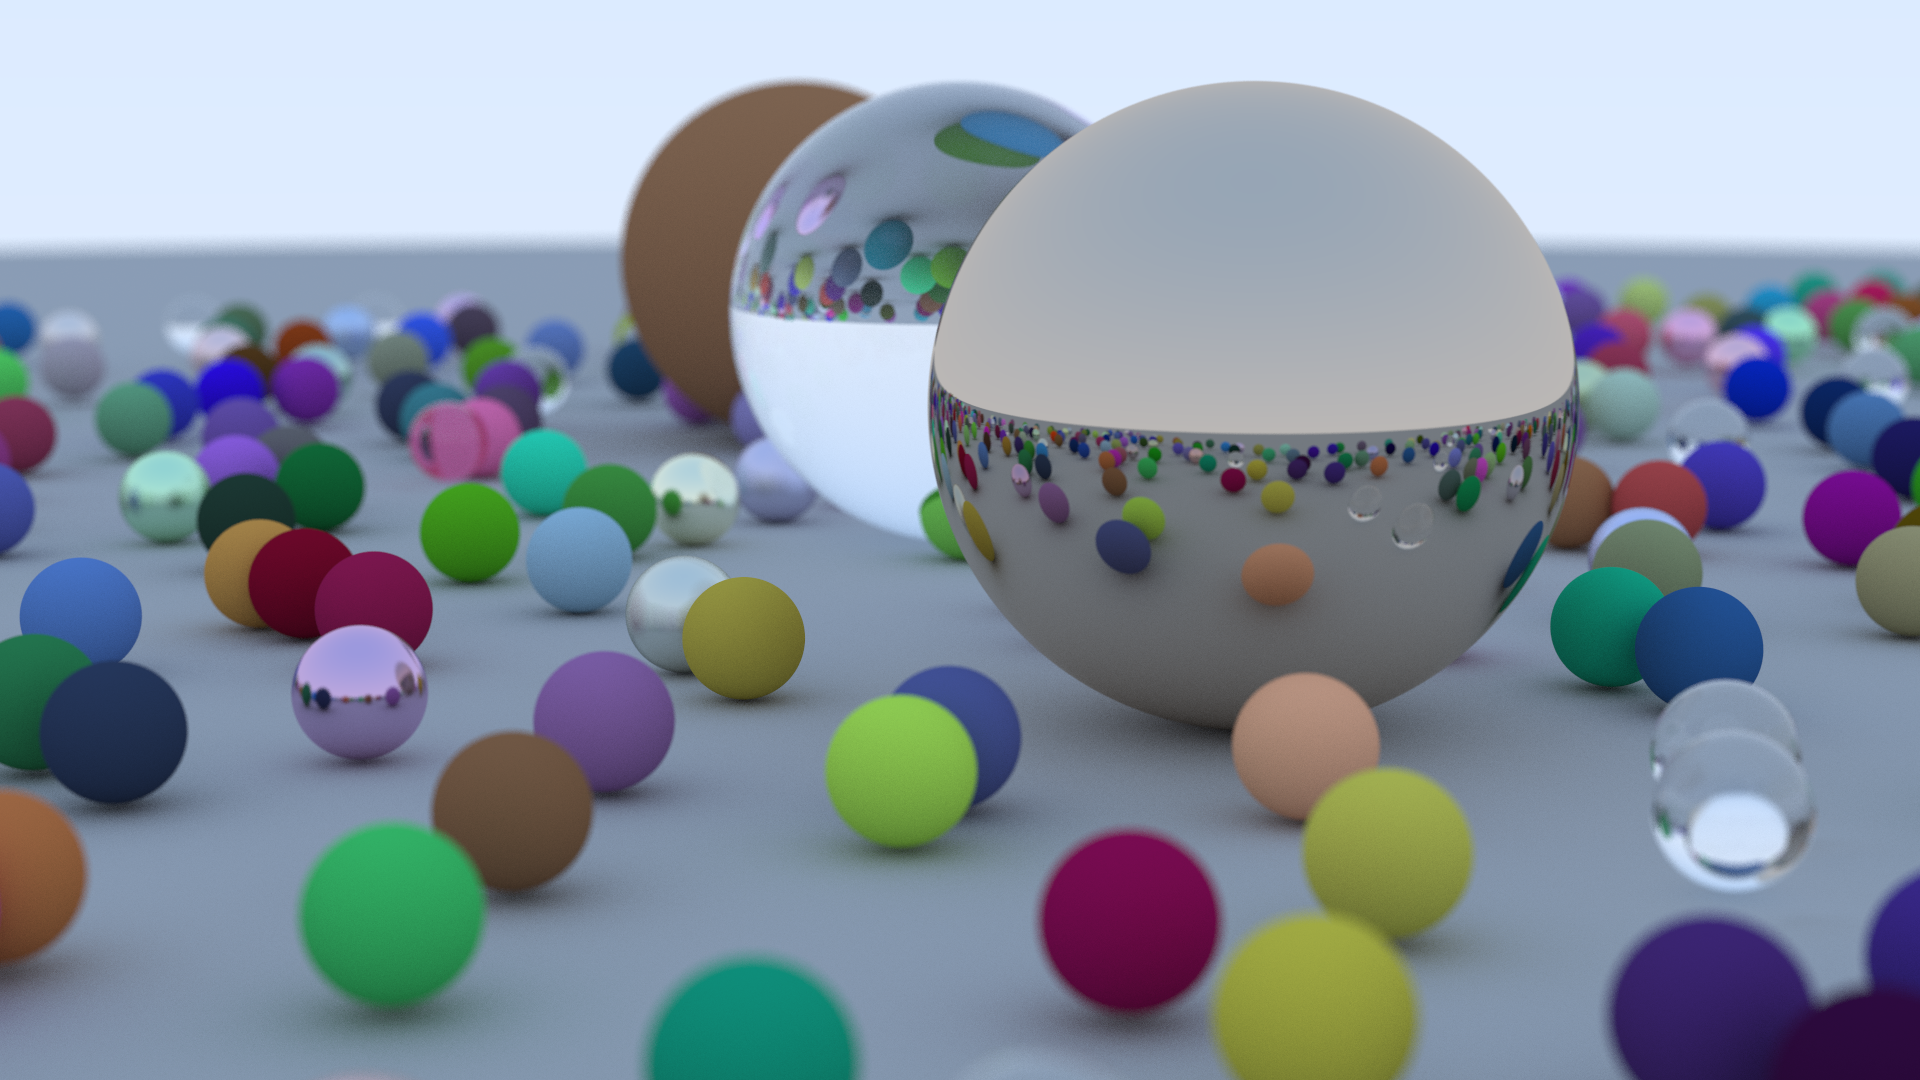
\includegraphics[width=0.65\linewidth]{img/ray_traced_balls.png}
    \caption[Sample program output high-resolution]{Example of program output, 1920 width, 300 samples per pixel and 200 max depth}
    \label{fig:ray_traced_max}
\end{figure}

And this is an example of the same picture, but with the settings used to test the programs on the personal laptop and server, which takes 168x more time than \autoref{fig:ray_traced_max}

\begin{figure}[h]
    \centering
    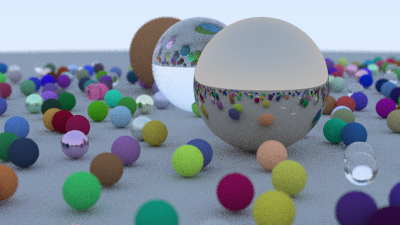
\includegraphics[width=0.65\linewidth]{img/regular_spheres_output.png}
    \caption[Sample program output default configuration]{Example of program output, 400 width, 50 samples per pixel and 50 max depth}
    \label{fig:ray_traced_average}
\end{figure}

\section{Running the program}
\label{sec:running_program}
To run the program, I have designed a \texttt{Makefile} that allows to run the program with different parameters, such as the number of cores to be used and where the user can specify the platform the benchmark is being run on. This is specially needed for macOS, as it needs \gls{sudo} privileges.

\begin{lstlisting}[caption={Makefile for running the program.}, label={lst:makefile_run}]
# ====== Configuration ======
CORES                 ?= 14
MAC_OS                ?= False
SERVER                ?= False
RESULTS_DIR           := $(CURDIR)/results-$(CORES)
SPHERE_DATA           := sphere_data.txt
POWERMETRICS_PID_FILE := $(RESULTS_DIR)/power/powermetrics.pid
POWER_LOG             := $(RESULTS_DIR)/power/powermetrics
POWER_TRIMM_LOG       := $(RESULTS_DIR)/power/powermetrics_trimmed
POWER_CLEANED_LOG     := $(RESULTS_DIR)/power/powermetrics_cleaned
POWER_INTERVAL        := 100  # Interval for powermetrics
PERF_COMMAND := perf stat -r 5 -e 'power/energy-pkg/,power/energy-ram/'

# ====== Directory Setup ======
$(RESULTS_DIR):
	@mkdir -p $(RESULTS_DIR)

# ====== Power Management Functions ======
# Args: $(1)=output_name
define start_powermetrics
	...
endef

# Args: $(1)=output_name
define stop_powermetrics
	...
endef

# ====== Ray Tracer Execution Functions ======
# Generic function to run a ray tracer with timing
# Args: $(1)=directory, $(2)=description, $(3)=command, $(4)=output_name
define run_raytracer
	...
endef

# Single-threaded version
# Args: $(1)=directory, $(2)=description, $(3)=command, $(4)=output_name
define run_raytracer_single
	...
endef

# ====== Build Functions ======
define build_cpp
	@echo "Building C++ ray tracer ..."
	...
endef

define build_go
	@echo "Building Go ray tracer ..."
	...
endef

# ====== Language-Specific Targets ======
# Python Implementations
.PHONY: python python-single pypy pypy-single
python: $(RESULTS_DIR)
	...

python-single: $(RESULTS_DIR)
	...

pypy: $(RESULTS_DIR)
	...
    
pypy-single: $(RESULTS_DIR)
	...
    
# C++ Implementations
.PHONY: cpp cpp-single cpp-build
cpp-build:
	...

cpp: cpp-build $(RESULTS_DIR)
	...
    
cpp-single: cpp-build $(RESULTS_DIR)
	...
    
# Go Implementations
.PHONY: go go-single go-build
go-build:
	...

go: go-build $(RESULTS_DIR)
	...
    
go-single: go-build $(RESULTS_DIR)
	...
    
# ====== Batch Operations ======
.PHONY: all all-multi all-single benchmark

all-multi: cpp go pypy python $(RESULTS_DIR)
	...

all-single: cpp-single go-single pypy-single python-single $(RESULTS_DIR)
	...

all: all-multi all-single
	...

benchmark: all
	...

# ====== Utility Targets ======
.PHONY: ppm-diff clean-power

ppm-diff:
	...

clean-power:
	...

# ====== Cleanup Targets ======
.PHONY: clean clean-builds clean-all stop-power
stop-power:
	...

clean:
	...

clean-builds:
	...

clean-all: clean clean-builds
	...

# ====== Help and Information ======
.PHONY: help info
help:
	...

info:
	...
\end{lstlisting}

When running the macOS version, the output has to be cleaned up, as the powermetrics command outputs a lot of information that is not needed for the report. This is done by running the \texttt{utilities/clean\_macos.sh} script inside the \texttt{results-<cores>} folder. Then, to get the power consumption, the \texttt{utilities/macos\_to\_jules.py} script has to be executed like this:
\begin{lstlisting}[language=bash, caption={Running the power consumption script.}, label={lst:macos_power_script}]
python3 macos_to_jules.py \
    '<output-folder>/powermetrics_cleaned_<lang>.log'
\end{lstlisting}

and the result would be printed to the terminal like this:
\begin{lstlisting}[language=bash, caption={Power consumption output.}, label={lst:macos_power_output}]
Power Statistics:
Average: 31707.79 mW
Maximum: 42631.00 mW
Minimum: 2342.00 mW

Energy Results:
Total energy: 50.605626 J
Total time: 1.60 s
Average power: 31707.79 mW
\end{lstlisting}